En este capítulo se describen brevemente las tecnologías
software en las que nos hemos apoyado para desarrollar el sistema propuesto
en este Trabajo Fin de Grado. Nos ayudará a situarnos en contexto para siguientes capítulos en los que abordaremos en mayor profundidad la utilidad que nos ha aportado cada una de ellas.

\section{Lenguaje visual Scratch}
\label{sec:scratch}
Scratch\footnote{\url{https://scratch.mit.edu/}} es un proyecto del Grupo Lifelong Kindergarten del MIT Media Lab.
Es utilizado por estudiantes y docentes de todo el mundo para programar animaciones, juegos e interacciones, fácilmente programables con su interfaz visual.\\

El nombre proviene de la palabra \textit{scratching} que en el mundo de la informática se refiere a reutilizar código, el cual puede ser usado de forma beneficiosa y efectiva para otros propósitos y fácilmente combinado, compartido y adaptado a nuevos escenarios, lo cual es una característica clave de Scratch.\\

Se trata de un lenguaje visual de programación donde los programas se construyen ensamblando bloques gráficos. Cada uno de estos bloques gráficos sería el equivalente a una función o método de cualquier lenguaje de programación.\\

Scratch 1.0, lanzada el 8 de enero de 2007, fue la primera versión de Scratch disponible para el público, esta primera versión disponía de un entorno muy limitado en cuanto a bloques funcionales. Esto fue mejorando en sus siguientes versiones hasta llegar a la 1.4, donde se decide reestructurar la herramienta, y crearla de nuevo desde cero debido a las limitaciones que estaban encontrando.\\

La segunda versión, la usada actualmente y por la que se popularizó, siguiendo a Scratch 1.4. Cuenta con un editor y un sitio web rediseñados, y permite al usuario editar proyectos directamente desde su navegador web, así como en un editor offline.\\

Se lanzó oficialmente en 2013 y ha sido completamente reescrito en Adobe Flash además debido a las nuevas características y al diferente lenguaje de programación, los proyectos de Scratch se guardan en formato .sb2. Esta es la versión que soporta actualmente la herramienta Scratch4Robots 1.0 y que seguiremos soportando en su versión mejorada Scratch4Robots 2.0\\

Scratch se define por una interfaz intuitiva y de simple manejo compuesta por tres zonas claramente diferenciadas. En la zona izquierda tendremos un escenario y un selector de \textit{sprites}, en el centro encontramos las diferentes categorías de bloques que podemos utilizar y un listado de los bloques pertenecientes a la categoría seleccionada, y por último tendremos un espacio vacio en la parte derecha en la que crearemos nuestro proyecto, con el simple movimiento de arrastrar el bloque deseado.\\

Tendremos bloques de las siguientes categorías:
\begin{itemize}
\item \textbf{Movimiento}: Mueve objetos y cambia ángulos.	  	 	
\item \textbf{Eventos}: Contiene manejadores de eventos situado al principio de cada grupo de instrucciones.
\item \textbf{Apariencia}: Controla el aspecto visual del objeto, añade bocadillos de habla o 
pensamiento, cambia el fondo, ampliar o reducir.	 	
\item \textbf{Control de flujo}: Sentencian condicionales y bucles. 
\item \textbf{Sonido}: Reproduce ficheros de audio y secuencias programables.	 	
\item \textbf{Sensores}: Los objetos pueden interactuar con el ambiente que ha creado el usuario.
\item \textbf{Lápiz}: Control del ancho, color e intensidad del lápiz.	 	
\item \textbf{Operadores} Operadores matemáticos, generador aleatorio de números, operadores booleanos.
\item \textbf{Datos}: Creación de variables y listas.	 	
\item \textbf{Mas Bloques}: Dispositivos o bloques externos creados por el usuario.
\end{itemize}

Al ser una herramienta madura y muy extendida existe una gran comunidad con la que compartir y de la que obtenter proyectos.

\begin{figure}[H]
    \centering
    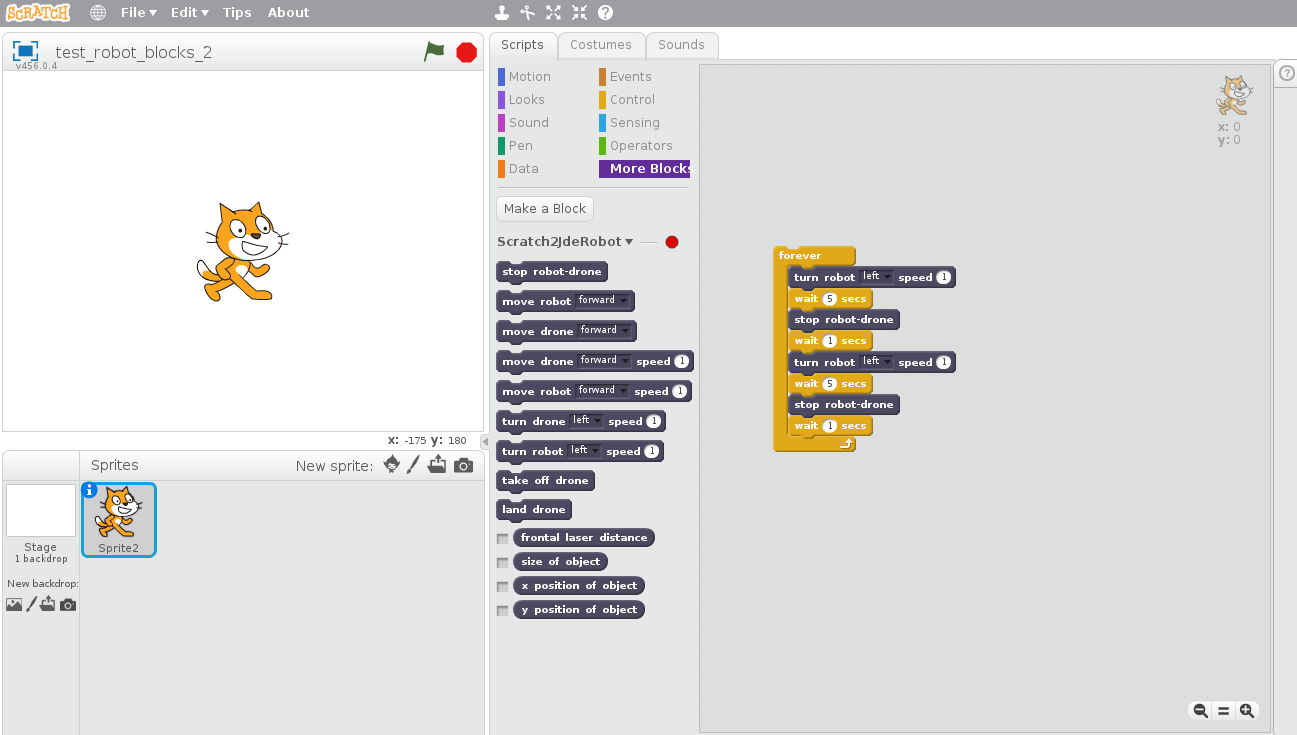
\includegraphics[scale=0.32]{img/scratch_IDE.png}
  	\caption{Espacio de trabajo de Scratch 2.0}
  	\label{fig:gazebo}
\end{figure}

Scratch sigue en constante evolución, existiendo la versión 3.0\footnote{\url{https://en.scratch-wiki.info/wiki/Scratch_3.0}} en fase \textit{Beta}. Esta versión está basada en la tecnología Blockly de Google, es capaz de integrarse en tablets, aumento de bloques funcionales, y un nuevo sistema de extensiones que permite el uso de servicios web. Aumenta su usabilidad con la agregación de una gran cantidad de videotutoriales y guías de iniciación en lenguajes de programación visual. Además todos los proyectos soportados por sus versiones anteriores no quedarán obsoletos, sino que podrán seguir funcionando en esta nueva versión, únicamente añadiendo funcionalidades.\\

Esta versión saldrá de forma oficial en Enero de 2019. Scratch 3.0 está escrito en HTML5, basado en web HTML, CSS y Javascript. Scratch 3.0 utilizará principalmente las bibliotecas WebGL, Web Workers y Web Audio Javascript. Javascript es un lenguaje ampliamente soportado en todos los navegadores web, y se eligió a WebGL por su velocidad y capacidades. A diferencia de Adobe Flash, usado para Scratch 2.0, Javascript funciona sin necesidad de complementos. En esta versión se sigue manteniendo su versión offline.\\

Es una de las herramientas fundamentales en nuestro trabajo, serán a los proyectos generados en lenguaje de programación visual, a los que realicemos la traducción a nodos ROS escritos en Python con nuestra herramienta Scratch4Robots.

\section{Lenguaje Python}
\label{sec:python}
 
Python\footnote{\url{https://www.python.org/}} es un lenguaje de programación administrado por la Python Software Foundation. Posee una licencia de código abierto, denominada Python Software Foundation License.\\

Es un lenguaje interpretado, por lo que no se necesita compilar el código fuente para poder ejecutarlo, esto ofrece ventajas como la rapidez de desarrollo e inconvenientes como una menor velocidad, en ciertos casos, cuando se ejecuta por primera vez un código, se producen unos bytecodes que se guardan en el sistema y que sirven para acelerar la compilación implícita que realiza el intérprete cada vez que se ejecuta el mismo código. \\

Lenguaje muy popular en los últimos años gracias a la cantidad de librerías que contiene, tipos de datos y funciones incorporadas en el propio lenguaje, que ayudan a realizar muchas tareas habituales sin necesidad de tener que programarlas desde cero, ademas cuya filosofía hace hincapié en una sintaxis que favorezca un código legible, facilitando su aprendizaje.\\

Su sintaxis muy visual, gracias a una notación indexada (con márgenes) de obligado cumplimiento. En muchos lenguajes, para separar porciones de código, se utilizan elementos como las llaves o las palabras clave begin y end. Para separar las porciones de código en Python se debe tabular hacia dentro, colocando un margen al código que iría dentro de una función o un bucle. Esto ayuda a que todos los programadores adopten unas mismas notaciones y que los programas de cualquier persona tengan un aspecto muy similar.\\

Se trata de un lenguaje de propósito general y multiplataforma, Aunque originalmente se desarrolló para Unix actualmente cualquier sistema es compatible con el lenguaje siempre y cuando exista un intérprete programado para él.\\

Pese a ser un lenguaje multiparadigma, principalmente está orientada a objetos lo que permite en muchos casos crear programas con componentes reutilizables. También permite programación imperativa y programación funcional por lo que se adapta al estilo del programador y no al revés.\\

En este Trabajo de Fin de Grado usamos la versión 2.7, existiendo también en su versión 3.0, y es el lenguaje en el que basamos todo el desarrollo realizado tanto para la  la propia generación del Nodo ROS, que estará desarrollado en Python, como para la traducción de bloques Scratch, cuya lógica sera en su totalidad en este lenguaje.\\

\section{Herramienta Scratch4Robots 1.0}
Scratch4Robots 1.0\footnote{\url{https://github.com/TheRoboticsClub/colab-gsoc2017-RaulPerula}} desarrollado por Raúl Pérula-Martínez durante el Google Summer of Code 2017, ofrece la capacidad de traducción de bloques Scratch a código Python.\\

La extensión de bloques que aporta a Scratch, realizan funcionalidades básicas de movimientos tanto para drones como para robots, disponiendo de un bloque por cada tipo de movimiento a realizar, movimientos en el eje X, eje Y o movimientos de rotación. Esto abarcaba la gama de movimientos de cualquier robot, pero dificultaba la integración de movimientos complejos ya que únicamente admite el movimiento en uno de los ejes a la vez.\\

En cuanto a traducción de bloques propios de Scratch, fuera del ámbito robótico, soporta ciertos bloques de control de flujo de programación para realizar funciones básicas como son un bucle infinito, bucles for, y sentencias condicionales.\\

Además el código generado a partir de la herramienta estaba basada en comunicaciones ICE, para el envió y obtención de información con el robot final.\\

\section{Biblioteca Kurt}
\label{sec:kurt}
Kurt\footnote{\url{https://en.scratch-wiki.info/wiki/Kurt}} es una biblioteca de Python que permite la manipulación compleja de proyectos de Scratch (archivos .sb y .sb2) a través de simples comandos de Python. Incluye un compilador y decompilador, que permite que un proyecto se cargue en un conjunto de objetos Python, y un compilador que permite cargar un conjunto de scripts de imágenes o texto en proyectos.\\

Al ser capaz de extraer toda la información contenida en un proyecto Scratch, y debido al parecido en la sintaxis de Scratch con Python nos sirve como principal fuente de recursos a la hora, por ejemplo, de realizar una transcripción de un bloque de Scratch a una sentencia Python.\\

En este Trabajo de Fin de Grado nos hemos basado en una versión\footnote{\url{https://pypi.org/project/jderobot-kurt/}} modificada de esta herramienta, capaz de admitir bloques definidos en extensiones externas de Scratch.\\

Se tratará con más profundidad el funcionamiento de esta librería en siguientes capítulos.




\section{Plataforma JdeRobot}
\label{sec:jderobot}
JdeRobot\footnote{\url{https://jderobot.org}} es una suite de desarrollo de software de robótica, domótica y sistemas de
visión computerizados cuya última versión, la 5.6, es la usada en este proyecto y permite la integración con ROS Kinetic. Proporciona un entorno distribuido donde las aplicaciones se forman mediante una colección de componentes asíncronos concurrentes, que se conectan mediante el middleware de comunicación ICE o mensajes ROS.\\

Se compone de interfaces, drivers, utilidades y aplicaciones para el desarrollo de cualquier proyecto de robótica. En este proyecto nos ayudamos de librerías como pueden ser \textit{comm, Config, JdeRobotTypes} que nos ayudan a agilizar el desarrollo de nuestra herramienta, abstraernos de ciertos niveles de complejidad y hacemos uso de una cantidad de entornos simulados en Gazebo con los que probar el correcto funcionamiento.\\

Nos hemos apoyado en esta plataforma para el desarrollo de este trabajo, usando diversas de sus librerías y entornos simulados predefinidos.


\subsection{Librería Comm}
\label{sec:libreria-com}
Librería desarrollada por JdeRobot con versiones tanto en Python como en C que nos abstrae del tipo de comunicación utilizada por nuestros componentes. Apoyándose en las librerías ya definidas en JdeRobot para el fácil uso de nodos ROS y Ice crea una capa de abstracción que permite que una aplicación sea capaz de funcionar tanto con \textit{ROS} como con comunicación \textit{Ice} sin necesidad de modificar el código interno de esta. De esta forma se aprovecha el trabajo anterior, se economiza tiempo, y se reduce el código redundante.\\

Su funcionamiento se apoya en el uso de un fichero de configuración necesario para establecer el tipo de comunicación que usaran los sensores y actuadores de nuestro robot. De este fichero obtendremos el tipo de comunicación y toda la información necesaria para poder establecerla. \\

Se trata de un paso más en la reducción de complejidad a la hora de programar algo tan complejo como un robot.\\

Para nosotros esta librería es el punto de partida a la hora de buscar que nuestra librería sea totalmente funcional con ROS, nos apoyamos en ella para el desarrollo de los componentes que hacen uso de comunicaciones ROS. Desacoplando y reutilizando algunas funciones de la librería referidas puramente a ROS.


\section{Entorno ROS}
\label{sec:ros}
ROS\footnote{\url{http://www.ros.org/}}(Robot Operating System) es un entorno para el desarrollo de software para robots que provee la funcionalidad de un sistema operativo en un clúster heterogéneo. Gestionado por Open Robotics Foundation. Proporciona bibliotecas y herramientas para ayudar a los desarrolladores de software a crear aplicaciones de robots. Proporciona abstracción de hardware, controladores de dispositivo, bibliotecas, visualizadores, paso de mensajes, administración de paquetes y más.\\

Es completamente de código abierto (BSD) y gratuito para que otros lo usen, cambien y comercialicen. Su objetivo principal es permitir que los desarrolladores de software creen aplicaciones de robots más capaces de forma rápida y fácil en una plataforma común. \\

En este trabajo vamos a utilizar la versión de ROS desarrollada para Ubuntu 16.04, ROS Kinetic\footnote{\url{http://wiki.ros.org/kinetic}}. Parte fundamental de este Trabajo Fin de Grado ya que uno de sus objetivos últimos es la generación de nodos ROS a partir de un proyecto programado en el lenguaje visual Scratch, además de la paquetización de la herramienta en una aplicación ROS. A continuación vamos a describir a muy alto nivel los conceptos básicos en los que se basa su arquitectura, esto nos va a ayudar a el proceso de funcionamiento de la herramienta Scratch4Robots 2.0.\\


\subsection{Maestro ROS}
El Maestro permite que todas las demás piezas de software de ROS (Nodos) encuentren y hablen entre sí. Sin el Maestro, los nodos no podrían encontrarse, intercambiar mensajes o invocar servicios. Proporciona registro y búsqueda de nombres para el resto del gráfico de computación.

\subsection{Nodos}
Algunos robots llevan varias computadoras, cada una de las cuales controla un subconjunto de los sensores o actuadores del robot. Incluso dentro de una sola computadora, a menudo es una buena idea dividir el software del robot en pequeñas partes independientes que cooperan para lograr el objetivo general. Para esto existen los nodos de ros.
Los nodos son procesos que realizan cálculos. ROS está diseñado para ser modular en una escala de grano fino, un sistema de control de robot generalmente comprende muchos nodos.
Por ejemplo, un nodo controla un láser, un nodo controla los motores de las ruedas, un nodo proporciona una vista gráfica del sistema y así sucesivamente.

\subsection{Servidor de Parámetros}
El servidor de parámetros permite que los datos se almacenen por clave en una ubicación central. Actualmente es parte del Máster.

\subsection{Mensajes}
Los nodos se comunican entre sí al pasar mensajes. Un mensaje es simplemente una estructura de datos, que comprende campos tipados. Los tipos primitivos estándar (entero, punto flotante, booleano, etc.) son compatibles, al igual que las matrices de tipos primitivos. Los mensajes pueden incluir estructuras y matrices anidadas arbitrariamente (al igual que las estructuras C).

\begin{figure}[H]
    \centering
    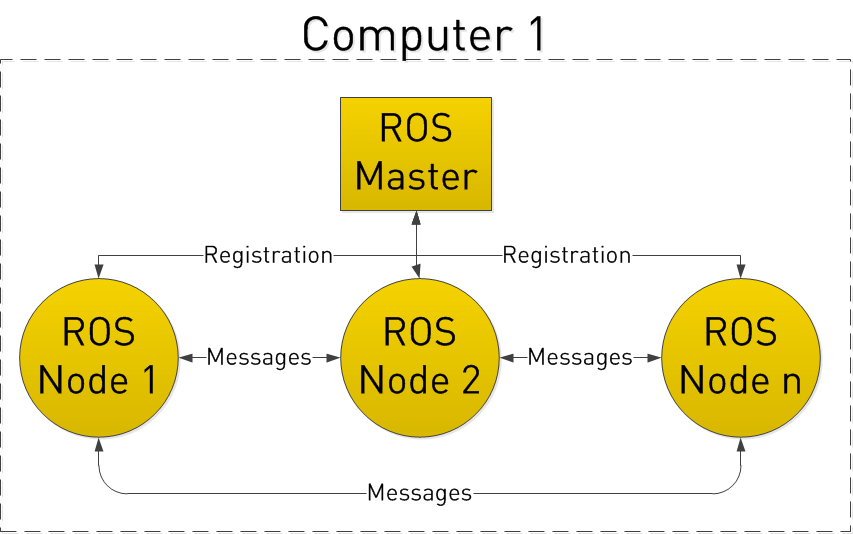
\includegraphics[scale=0.45]{img/ros-architecture.png}
  	\caption{Arquitectura básica ROS maestro-nodo}
  	\label{fig:ros-arch}
\end{figure}

\subsection{Topics o Temas}
Los mensajes se enrutan a través de un sistema de transporte con semántica de publicación suscripción. Un nodo envía un mensaje publicándolo en un tema determinado. El tema es un nombre que se usa para identificar el contenido del mensaje. Un nodo que está interesado en cierto tipo de datos se suscribirá al tema apropiado. Puede haber varios editores y suscriptores simultáneos para un único tema, y un solo nodo puede publicar y / o suscribirse a múltiples temas. En general, los editores y los suscriptores no conocen la existencia de los demás. La idea es desacoplar la producción de información de su consumo. Lógicamente, uno puede pensar en un tema como un bus de mensajes fuertemente tipado. Cada bus tiene un nombre, y cualquiera puede conectarse al bus para enviar o recibir mensajes, siempre que sean del tipo correcto.

\begin{figure}[H]
    \centering
    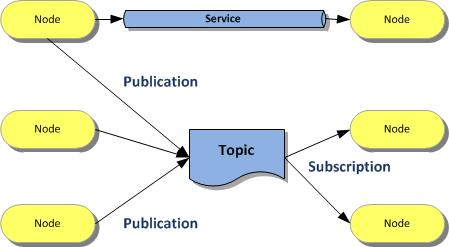
\includegraphics[scale=1]{img/ros-architecture-3.jpg}
  	\caption{Arquitectura básica ROS publicación-suscripción}
  	\label{fig:ros-servicio}
\end{figure}

\subsection{Servicios}
El modelo de publicación / suscripción es un paradigma de comunicación muy flexible, pero su transporte unidireccional de muchos a muchos no es apropiado para las interacciones de solicitud / respuesta, que a menudo se requieren en un sistema distribuido. La solicitud / respuesta se realiza a través de servicios, que están definidos por un par de estructuras de mensaje: una para la solicitud y otra para la respuesta. Un nodo proveedor ofrece un servicio con un nombre y un cliente usa el servicio enviando el mensaje de solicitud y esperando la respuesta. Las bibliotecas cliente de ROS generalmente presentan esta interacción al programador como si fuera una llamada de procedimiento remoto.\\

\section{Simulador Gazebo}
\label{sec:gazebo}
Gazebo\footnote{\url{http://gazebosim.org/}} es un simulador 3D para robots, es un proyecto de Open Source Robotics Fundation distribuido bajo la licencia Apache 2.0, con un motor de físicas y cinemáticas muy potente, es la principal herramienta en la que se apoya el desarrollador para verificar de forma segura que su implementación cumple con el objetivo determinado. Este tipo de simuladores han conseguido una fuerte evolución del mundo de la robotica ya que nos permite desarrollar componentes para dispositivos y robots complejos de forma barata y rápida.
Se trata de una herramienta altamente personalizable y moldeable que admite plugins que permiten una gestión más fina de los recursos de cara a conseguir una simulación más precisa o simplemente perimitir al desarrollador trabajar con mayor comodidad sobre el simulador.
Al ser un proyecto open source existe una comunidad muy activa detrás de esta herramienta compartiendo conocimientos y publicando nuevas funcionalidades de esta.
Cabe destacar que Gazebo se compone principalmente de un cliente y un servidor. El
servidor es el encargado de realizar los cálculos y la generación de los datos de los sensores,además de poder ser usado sin necesidad de una interfaz gráfica.
El cliente proporciona una interfaz gráfica basada en QT que incluye la visualización de la simulación y una serie de controles de multitud de propiedades. Esta configuración permite lanzar múltiples clientes sobre un servidor, consiguiendo múltiples interfaces de la misma simulación.
Destacar que en 2013, este simulador se utilizó en la Virtual Robotics Challenge, un componente del DARPA Robotics Challenge.
En este proyecto Gazebo se emplea para probar la solución desarrollada en un entorno controlado para después, pasar a un entorno real. \\

\begin{figure}[H]
    \centering
    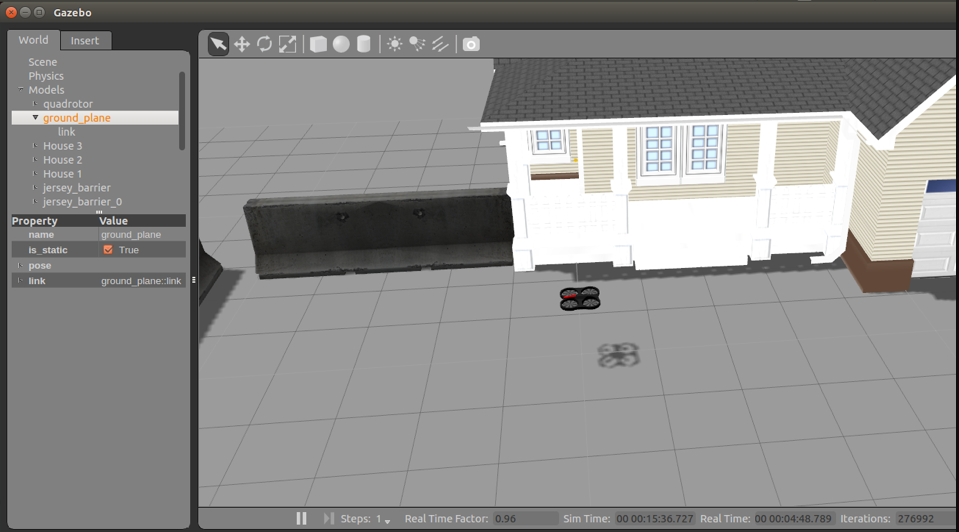
\includegraphics[scale=0.50]{img/gazebo.PNG}
  	\caption{Entorno de simulación Gazebo}
  	\label{fig:gazebo}
\end{figure}

En este proyecto se hace uso de la versión 7 de Gazebo, siendo el entorno simulado elegido para la validación de todos los desarrollos sobre robots simulados.